\section{Evaluation}
\label{sec:eval}

In this section we present an emperical evaluation of \quark on two
case studies. First is a collaborative document editing
application -- a common usecase addressed by several CRDT
proposals~\cite{rga, treedoc, crdts}. Second is a replicated key-value
store implemented using a mergeable Red-Black tree data structure.

\subsection{Collaborative Editing}

\quark's MRDT approach obviates the need to build a dedicated
replicated data type for collaboratively-edited documents; an ordinary
document format extended with a merge operation would suffice. While
many data structures exist to represent text documents (e.g.,
ropes~\cite{boehm95}), we decided to adopt the simplest representation
of a document as a list of characters. 
\begin{center}
\begin{ocaml}
        type doc = char list
\end{ocaml}
\end{center}
While being simple, the advantage of this presentation is that we can
simply reuse the three-way \C{List.merge} function of the list data
type to merge documents. \C{List.merge} is a simple implementation of
list merge algorithm (in ~60 lines of OCaml) inspired by the GNU
\C{diff3} algorithm~\cite{gnudiff}. We thus adopt a straightforward
approach to building a collaborative document editor with the
intention to keep the development effort low enough to be easily
replicated. The convergence guarantee of \quark ensures that the
simplicity of our implementation doesn't come at the expense of
correctness. The aim of the experimental evaluation is to quantify the
impact of \quark on the performance.

Our experiment setup consists of multiple collaborators simultaneously
editing a 10000+ line document obtained from the Canterbury
Corpus~\cite{canterbury}. Each user holds a replica of the document
and is assumed to be editing the document at the speed of 240
characters per minute or 1 character every 0.25s. At 6 characters per
word, this amounts to 40 words per minute, which is the average typing
speed of humans. Each edit is immediately persisted to the disk by
creating a new version in the backing store. Thus there are at least
as many versions of the document as there are edits. Such extensive
versioning may be considered excessive in practice and could be
disabled. Each user process runs a \quark thread that commits
user-generated document versions to the local branch, while
merging with the concurrent versions from the remote branches in the
background. Each merge is synchronized as described in previous
sections.

\quark's background merges however pose a new problem as they create
new versions on the local branch in the background while the user is
busy editing an older version. When the user attempts to write their
version of the document to the store, simply committing it would
effectively override the concurrent updates from other users obtained
via background merges. The solution, fortunately, is straightforward:
we \emph{merge} the user-submitted value with the (value of) the
latest version on the local branch to create a new version that
includes the updates from either direction. Since this merge is fully
confined to the local replica, it is guaranteed to not affect the LCA
of the local branch with respect to a remote branch. To the external
world, it appears as if the local branch has simply committed a new
version.
% The LCA for this merge is
% simply the last version on the local branch read by the user. This
% merge need not be synchronized as it doesn't alter the LCAs between
% any two branches. The merged value can then returned to the user as
% the result of the write.
Thus, \quark's \C{write} is a function of type $\texttt{Value}
\rightarrow \texttt{Value}$, where $\texttt{Value}$ is \C{doc} in the
current application.

\noindent\paragraph{Latency} To measure the impact of \quark runtime on user
writes, we measure the latency of the \C{write} operation, which
includes the time spent merging the user version with the current
version, and persisting the resultant version to the store. We conduct
the experiments on a three-node cluster of \C{i3.large} machines in
Amazon \C{us-west2} data center. Each user connects to one of the
machines, forks a new branch, and performs 1000 edits in succession,
saving the document after each edit. We progressively increase the
number of concurrent users editing the document from 3 to 200 and
measure the impact of the increased concurrency on write latency.
Fig.~\ref{fig:latency} shows the 10th, 50th (median), and 90th
percentile latency values. The median and 10th percentile latencies
remain more-or-less constant with a slight increase between 3 and 60
concurrent users. This demonstrates that \quark has negligible effect
on the per-operation latency, which is expected. The 90th percentile
latency, however, shows no clear pattern by the virtue of being more
susceptible to transient system conditions. Nonetheless, the maximum
value of 90th percentile latency measured (32ms) remains well below
the the time between consecutive edits (0.25s), making it hard to
perceive by a human user. 

\begin{figure}[ht]
  \centering
    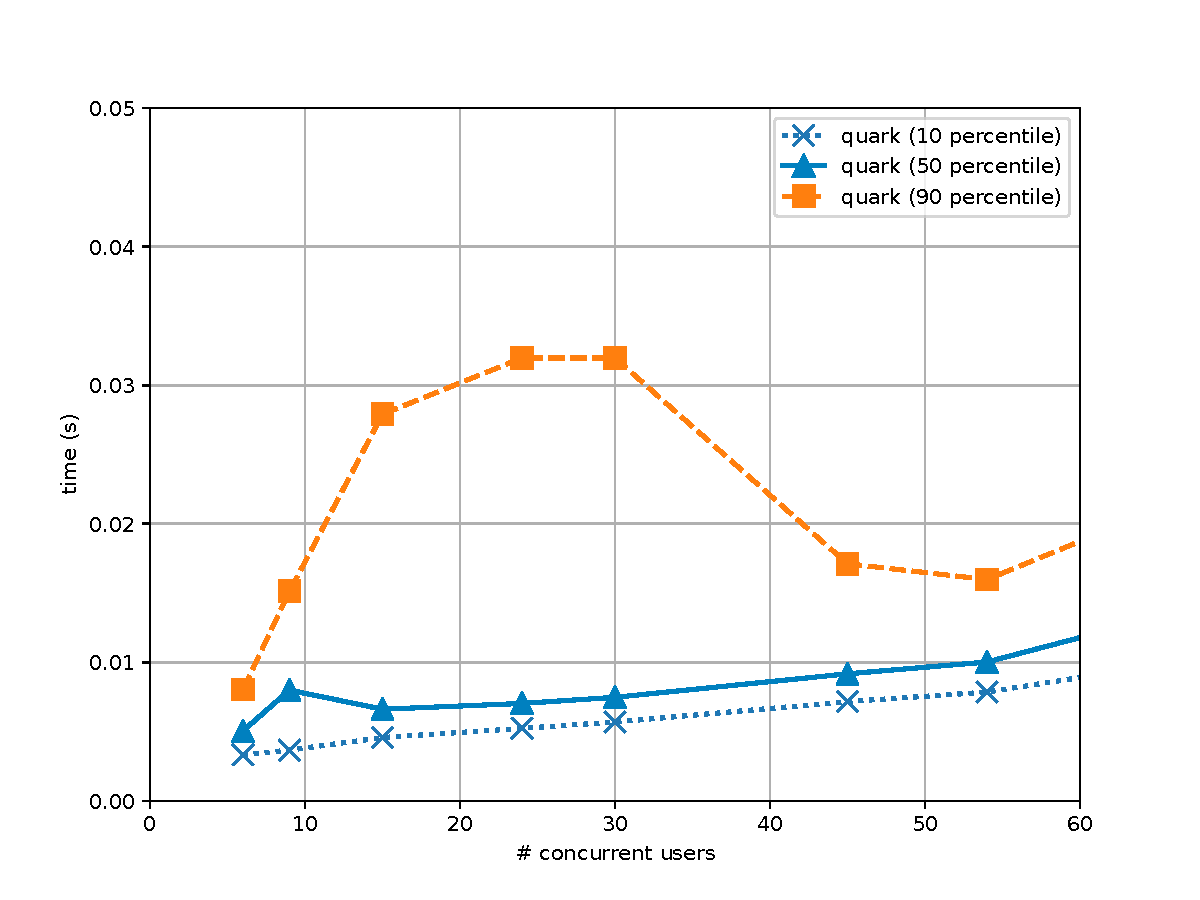
\includegraphics[scale=0.4]{Figures/monkey_latency}
\caption{Latency of writes to a shared document under \quark. }
\label{fig:latency}
\end{figure}


For comparison against a baseline, we have implemented an ``SC''
approach which achieves convergence by synchronizing each operation,
i.e., executing it under strong consistency (SC). The SC
implementation shares most of its code with \quark with the only
change being that it wraps commits instead of merges inside a lock.
As with \quark, we measured the write latency of the SC implementation
while increasing the number of concurrent users ($n$).  The median SC
write latency increases super-linearly from 10ms for $n=3$ to 63s
(i.e., >1m) for $n=60$, which is considerably more than the inter-edit
latency of 0.25s.


\noindent\paragraph{Staleness} Our implementation of \quark relies on
Scylla to replicate the contents of each branch across all the
replicas as fast as the network allows. However, for a user $A$ to see
the changes made by the other user $B$, the changes have to be
reflected in $A$'s local version, which can only happen through a
merge operation. Since \quark synchronizes merge operations globally,
it induces additional delay before $A$ can see $B$'s changes. We call
this additional delay \emph{staleness} as with the progression of
time, $B$'s version known to $A$ becomes increasingly stale. At the
system-level, an increase in staleness effectively delays the
convergence (but doesn't preempt it, as proved by
Theorem~\ref{thm:progress}). 

\begin{figure}[ht]
  \centering
    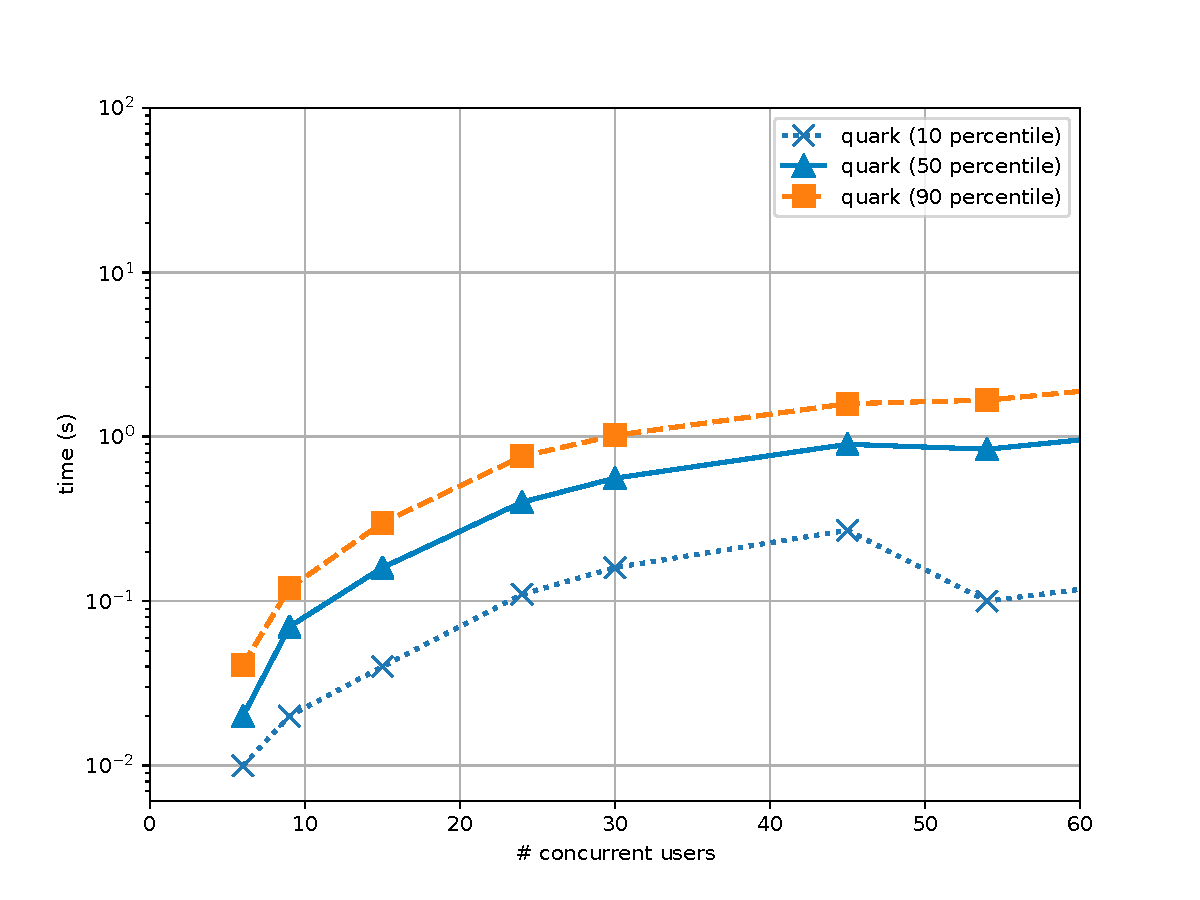
\includegraphics[scale=0.4]{Figures/monkey_staleness}
\caption{Staleness increases as the number of concurrent editors
  increase.}
\label{fig:monkey-staleness}
  \vspace*{-0.2in}
\end{figure}

To understand the effect of \quark on
staleness, we quantify and measure it along with latency in the
experiment setup described above. Staleness is defined as the time
taken for a version committed on one replica to be merged into a
concurrent version on a remote replica. To measure staleness, we
annotate every version $v$ with the timestamp $t$ of capturing the
wall clock time of its creation. When $v$ is is merged into a remote
branch $b$ at a later time $t'$, the difference $t' - t$ denotes the
staleness of $v$ w.r.t the new version on $b$. One such staleness
measurement is recorded for every merge that ever happens during the
experiment. We compute 10th, 50th, and 90th percentiles of staleness
values thus obtained. Fig.~\ref{fig:monkey-staleness} shows the
results. As evident, staleness increases steadily with the increasing
number of concurrent replicas, which is expected considering that
merges are synchronized, and increasing the number of replicas reduces
the number of opportunities for a replica to merge. The increase is
roughly linear in the number of replicas as our implementation passes
the lock around in a round-robin fashion, thus increasing the lock
latency in proportion to the number of replicas. Nonetheless, the 90th
percentile staleness values remain low -- in the order of 100ms with
the number of replicas under 30, and in the order of 1s with number of
replicas under 60. While further optimizations might reduce staleness,
a non-trivial staleness overhead is inevitable in \quark due to our
use of synchronized merges to guarantee convergence. 

% Our approach thus
% introduces staleness as novel tradeoff against convergence. While
% trading off staleness may not be an optimal choice for every
% application, it is arguably a less disruptive choice if an application
% has to choose between latency and staleness.
% Sec.~\ref{sec:motivation}\footnote{
%   Git admits anamolous version history graphs where two branches can
%   have the same set of commits and yet differ in their final version.
%   Supplementary material describes two such cases we observed on
%   Github.}. 

\subsection{Key-Value Store}

We repeat our experiments on a mergeable key-value store application
we implemented using a Red-Black tree MRDT. Latency results are shown
in Fig.~\ref{fig:rb-latency}, and staleness results in
Fig.~\ref{fig:rb-staleness}.

\begin{figure}[ht]
  \centering
    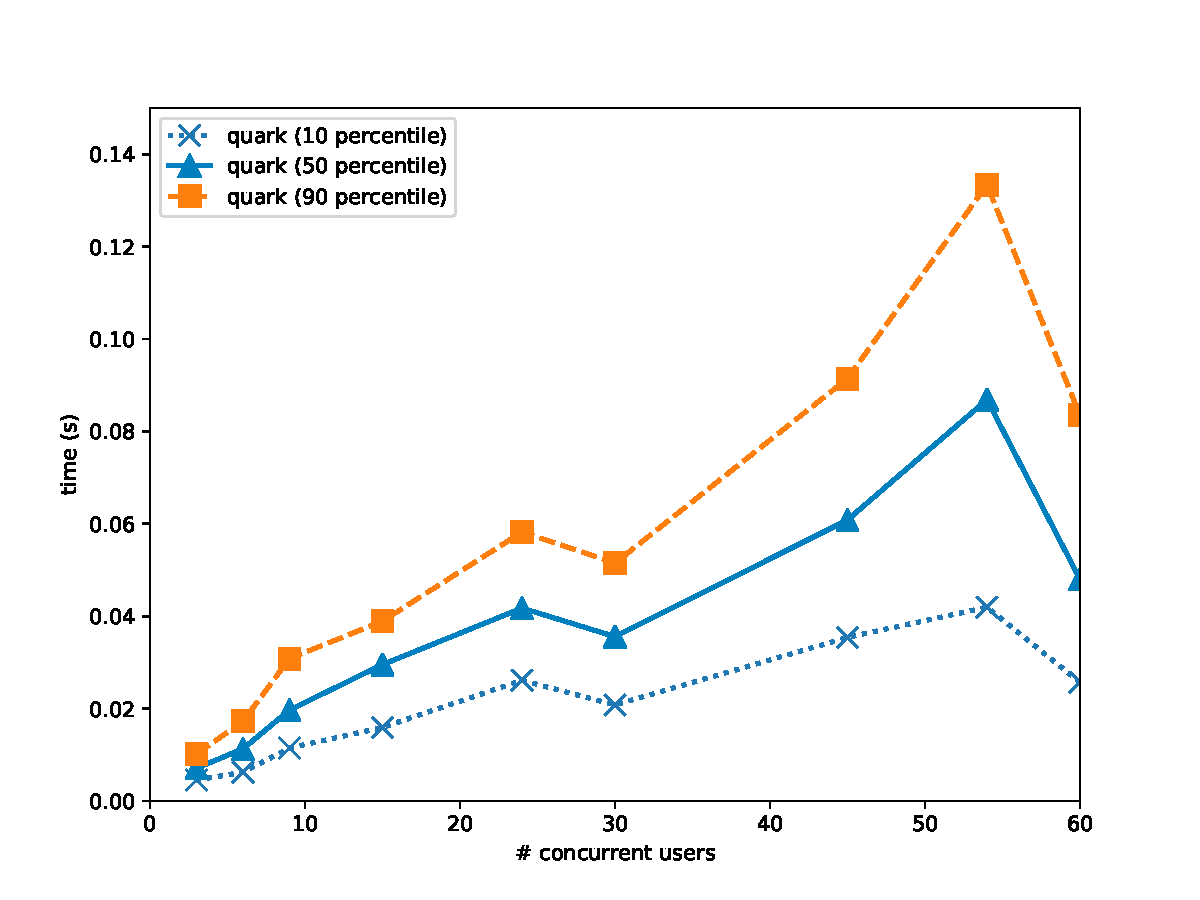
\includegraphics[scale=0.4]{Figures/rbmonkey_latency}
  \caption{Latency for Key-Value store operations under \quark}
\label{fig:rb-latency}
  \vspace*{-0.2in}
\end{figure}

\begin{figure}[ht]
  \centering
    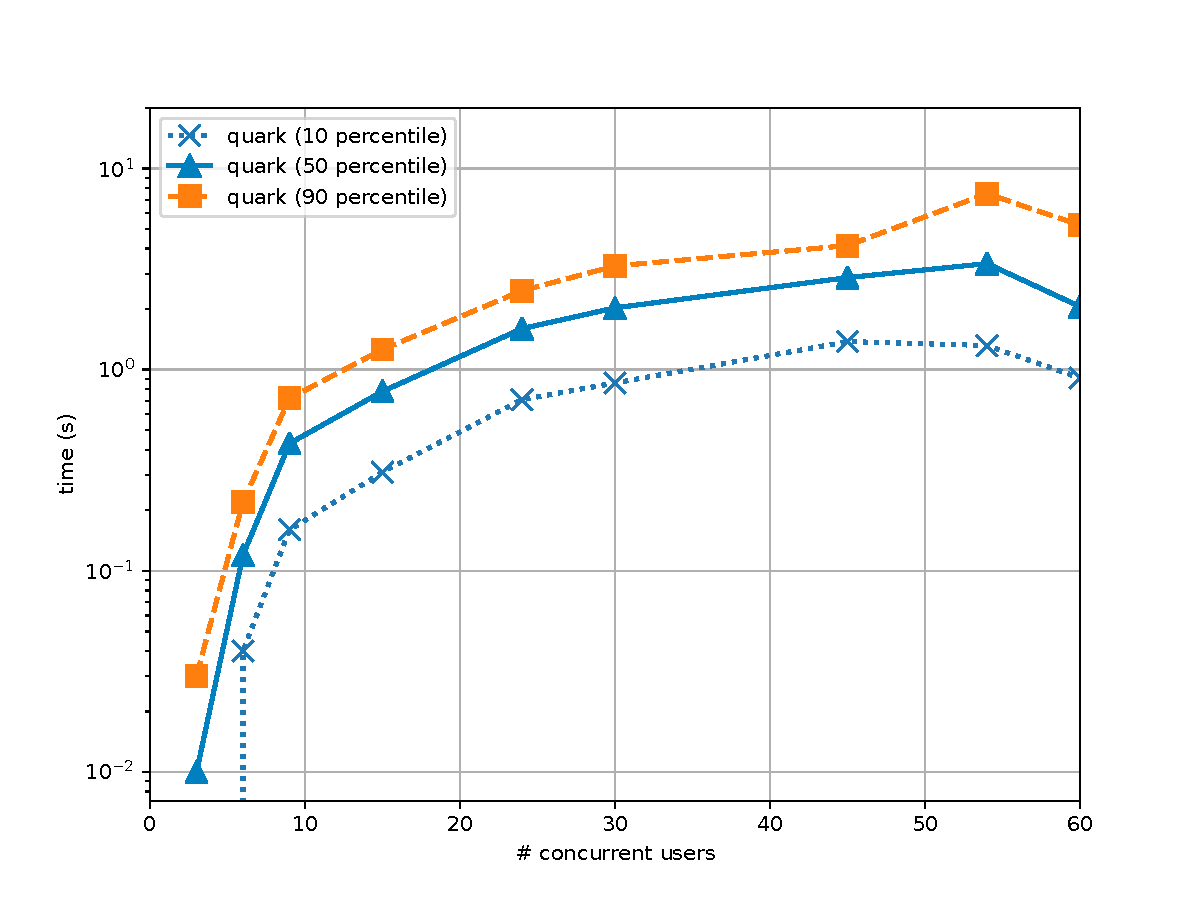
\includegraphics[scale=0.4]{Figures/rbmonkey_staleness}
  \caption{Key-Value store staleness under \quark}
\label{fig:rb-staleness}
  \vspace*{-0.2in}
\end{figure}

Our experiments bring to the fore an inherent tradeoff among the
competing concerns of RDTs, namely (\rom{1}). The ease of programming
convergence, (\rom{2}) Latency, and (\rom{3}).  Staleness. While CRDTs
try to optimize for latency and staleness, they require a significant
amount of development and verification effort to be expended to ensure
convergence~\cite{kleppmann2017}. In contrast, \quark lets developers
derive convergent-by-construction RDTs from ordinary data data types
that are optimized for latency, but incur a staleness overhead that
delays the time to convergence. 


